\documentclass{article}

% if you need to pass options to natbib, use, e.g.:
% \PassOptionsToPackage{numbers, compress}{natbib}
% before loading nips_2016
%
% to avoid loading the natbib package, add option nonatbib:
% \usepackage[nonatbib]{nips_2016}

%\usepackage{nips_2016}

% to compile a camera-ready version, add the [final] option, e.g.:
 \usepackage[final]{nips_2016}

\usepackage[utf8]{inputenc} % allow utf-8 input
\usepackage[T1]{fontenc}    % use 8-bit T1 fonts
\usepackage{hyperref}       % hyperlinks
\usepackage{url}            % simple URL typesetting
\usepackage{booktabs}       % professional-quality tables
\usepackage{amsfonts}       % blackboard math symbols
\usepackage{nicefrac}       % compact symbols for 1/2, etc.
\usepackage{microtype}      % microtypography
\usepackage{graphicx}

\title{Category Classification With Animal Image Data}

% The \author macro works with any number of authors. There are two
% commands used to separate the names and addresses of multiple
% authors: \And and \AND.
%
% Using \And between authors leaves it to LaTeX to determine where to
% break the lines. Using \AND forces a line break at that point. So,
% if LaTeX puts 3 of 4 authors names on the first line, and the last
% on the second line, try using \AND instead of \And before the third
% author name.

\author{
 Chudan Liu\\
 Department of Mathematics\\
 Harvey Mudd College\\
 Claremont, CA 91711 \\
 \texttt{iliu@g.hmc.edu} \\
 %% examples of more authors
  \And
  Xinyu Yang \\
  Department of Mathematics\\
  Harvey Mudd College \\
  Claremont, CA 91711 \\
  \texttt{xiyang@g.hmc.edu} \\
 %% \And
 %% Coauthor \\
 %% Affiliation \\
 %% Address \\
 %% \texttt{email} \\
}
\begin{document}
% \nipsfinalcopy is no longer used

\maketitle

\begin{abstract}
 
Image classification extracts the key features of images, analyzes the numerical properties of these features and classify the data into categories, which is one of the most important applications of deep learning to computer vision problems. Image classification, as a complex task for machines, has a wide range of application in real life, such as image retrieval, object detection, objection segmentation and object classification. This paper introduces multiple methods for object classification and evaluates the performance of each method through different experiments on species categories of animal image data. While image classification can be conducted through both supervised and unsupervised learning, we train an animal category predictor using logistic regression model, multilayer perceptrons neural network, support vector machines (SVM) with linear kernel and radial basis function kernel, which could be output and saved on disk. Then, we compare the performance of these predictors by computing their running time and accuracy through confusion matrices. With these models, we create an interactive animal classification that lays satisfying results in running time and validity scopes. 
\end{abstract}

\section{Introduction}
\paragraph{}
In this paper, we are dealing with image classification problem, which is the job of assigning an input image one label from a fixed set of categories. This is one of the core problems in Computer Vision that, despite its simplicity, has a large variety of practical applications. Moreover many other seemingly distinct Computer Vision tasks (such as object detection, segmentation) can be reduced to image classification. Thus, image classification problem is the foundation of most of the image-based big data problem, including optical character recognition, edge detection, and object recognition.
\paragraph{}
For this project, we selected the Common Object in Context (COCO) dataset $^{[1]}$, a popular image recognition, segmentation, and captioning dataset to perform image classification. We chose this dataset because it has over 80,000 images with multiple objects and clear labels. We specifically look into the animal supercategory, which has 10 categories of different animals. The main task is to use these images and animal labels as input to train a classifier that can perform prediction.
\paragraph{}
Many useful algorithms for image classification have been developed throughout these years. For our project, we chose several different algorithms to train the classifiers and use various methods to evaluate these algorithms. We primarily focused on the logistic regression model, multilayer perceptron neural network model, and support vector machine (linear and nonlinear kernel).
 
\paragraph{}
The major parts of this report are:
\begin{enumerate}
\item 
A summary of the algorithms we used in our project, with detail explanation and mathematical justification.
\item 
Extraction of the final dataset and training and testing data processing.
\item 
Performance analysis of each algorithm with an introduction to confusion matrix.
\item 
Experiment of how good each predictor actually works with several examples
\item 
Possible future work and applications
\end{enumerate}

\section{Learning Algorithms}
\paragraph{}
In our project, we used four algorithms to classify the data: Logistic Regression, multilayer perceptron neural network (MLP), linear support vector machines and nonlinear support vector machines with radial basis function kernel. Below are details about the algorithm and parameters we used in this project. 
\subsection{Multinomial Logistic Regression}
\paragraph{}
Multinomial Logistic Regression is the first learning algorithm we used. Given a set of independent categorical variables, which are the pixels of animal images from our dataset in this case, we trained a logistic regression model to predict the probabilities of the different possible animals of the independent  categorical variables.
\paragraph{}
As most other statistical classification models, the foundation of the logistic regression model is to construct a linear predictor function that computes a score from a set of regression coefficients  that indicate the relative effect of variables on the $y$. In particular, \[
Score(k, X_i) = \beta_k \cdot X_i,
\]
where $k$ indicates the outcome  $k$, which is the category ID; $X_i$ is the vector of explanatory variables, which are all the pixels of an image describing observation $i$; $\beta_k$ is a vector of  regression coefficients corresponding to outcome k. For all $X_i$, the predicted outcome falls in the outcome with the highest score. If we denote the probability that the $X_i$ falls in category $k$ as \[ \pi_{ik} = P\{Y_i = k\},
\]
since the categories are mutually exclusive and exhaustive, $\pi_{ij}$ add up to one for each individual  image and we have \[ 
\sum_{k=1}^K \pi_{ik} = 1 \ \textbf{ for all }  i \]
\paragraph{}
To approach the multinomial data, we will nominate one of the outcome categories as a baseline cell, calculate the log-odds for all other categories relative to the baseline, and let the log-odds be a linear function of the predictor Score function. We assume the log-odds of each outcome category follow a linear model \[
\eta_{ik} = log \ \frac{ \pi_{ik} }{ \pi_{iK} } = \alpha_k + x_i'\beta_k
\]
where $\alpha_k$ is a constant and $\beta_k$ is a vector of regression coefficients for $k \in [1, K-1]$.
We can see that the logits are a quadratic function and therefore we will entertain the model \[
\eta_{ik} = \alpha_k + \beta_k \alpha_i + \gamma_k a_i^2 \]
where $a_i$ is the midpoint of the $i^{th}$ image and $k = 1, 2$ for the category ID among all of them respectively.


\subsection{Multilayer Perceptron(MLP) Classifier}
\paragraph{}
Multilayer Perceptron (MLP) is a supervised learning algorithm with multiple hidden layers. It inputs a set of $m$ features \[
X = x_1, x_2, ... , x_m\] and an output function $f(X)$, learns a non-linear function approximator for either classification or regression.


\begin{center}
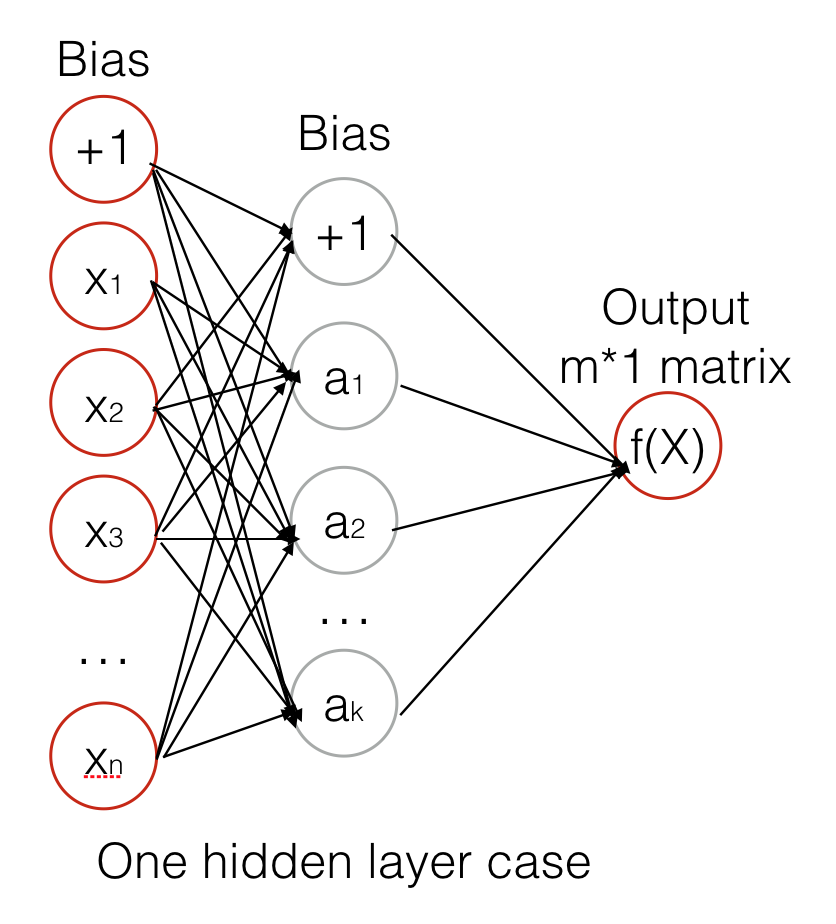
\includegraphics[scale=0.3]{2.png}
\end{center}
 
\paragraph{}
\textbf{Figure 1.} Signal flow graph of MLP. The input layer is (X), an m*n matrix, where m is the number of training sets and n is the number of features, which in our case is 256*256. In the middle, there are multiple hidden layers and each layer has a specific number of neutrons. 

 
\paragraph{}
The perceptron computes a single output from multiple real-valued inputs by forming a linear combination according to its input weights and then possibly putting the output through some nonlinear activation function. Mathematically, this can be written as 
\[ y = \varphi(\sum_{i=1}^n w_ix_i+b) = \varphi(w^Tx+b)
\]
where $w$ denotes the vector of weights, $b$ is the bias, and $\varphi$ is the activation function. The supervised learning problem of the MLP can be solved with the back-propagation algorithm. The algorithm consists of two steps. In the forward pass, the predicted category ID corresponding to the given image features are evaluated in the above equation. In the backward pass, partial derivatives of the cost function $\frac{\partial l}{\partial \theta}$  are propagated back through the network. The network weights can then be adapted using any gradient-based optimization algorithm. The whole process is iterated until the weights have converged$^{[5]}$.

\paragraph{}
As someone may ask, given the logistic regression model, why we need multilayer perceptrons to classify dataset. Comparing with logistic regression, the advantage of multilayer perceptrons is the capability to learn non-linear models. However, different random weight initializations can have different test accuracy because MLP with hidden layers have a non-convex loss function where there exists more than one local minimum. In actual implementation, we need to take into account the nonlinearity function, weight initialization, learning rate, number of hidden units, and regularization parameter.


\subsection{Linear Support Vector Machines}
\paragraph{}
Support Vector Machine (SVM) is a supervised machine learning algorithm that builds a hyperplane in a high dimensional space which can be used in classification problems. In this algorithm, we plot each data item as a point in $n$-dimensional space (where $n$ is the number of features in the image) with the value of each feature being the value of a particular coordinate. Then, we perform classification by finding the hyperplane that differentiates the two classes very well. Good separation is achieved by the hyperplane that has the largest distance to the nearest training data point of any class (functional margin).
\paragraph{}
However, in reality most of the datasets are not linearly separable. Hinge loss function can solve the problem,
\[ max(0, 1-y_i(\vec{w} \cdot \vec{x_i}-b))\]
where $y_i$ is the category for image $i$ $^{[2]}$. This function is zero if $\vec{x_i}$ lies on the correct side of the margin. For data on the wrong side of the margin, the function's value is proportional to the distance from the margin. Then the optimization problem becomes to minimize\[
[\frac{1}{n}\sum_{i=1}^n max(0,1-y_i(\vec{w} \cdot \vec{x_i}-b))]+\lambda ||\vec{w} ||^2 \]
where the parameter lambda determines the tradeoff between increasing the margin-size and ensuring that $x_i$ lie on the correct size of the margin$^{[3]}$. 
\begin{center}
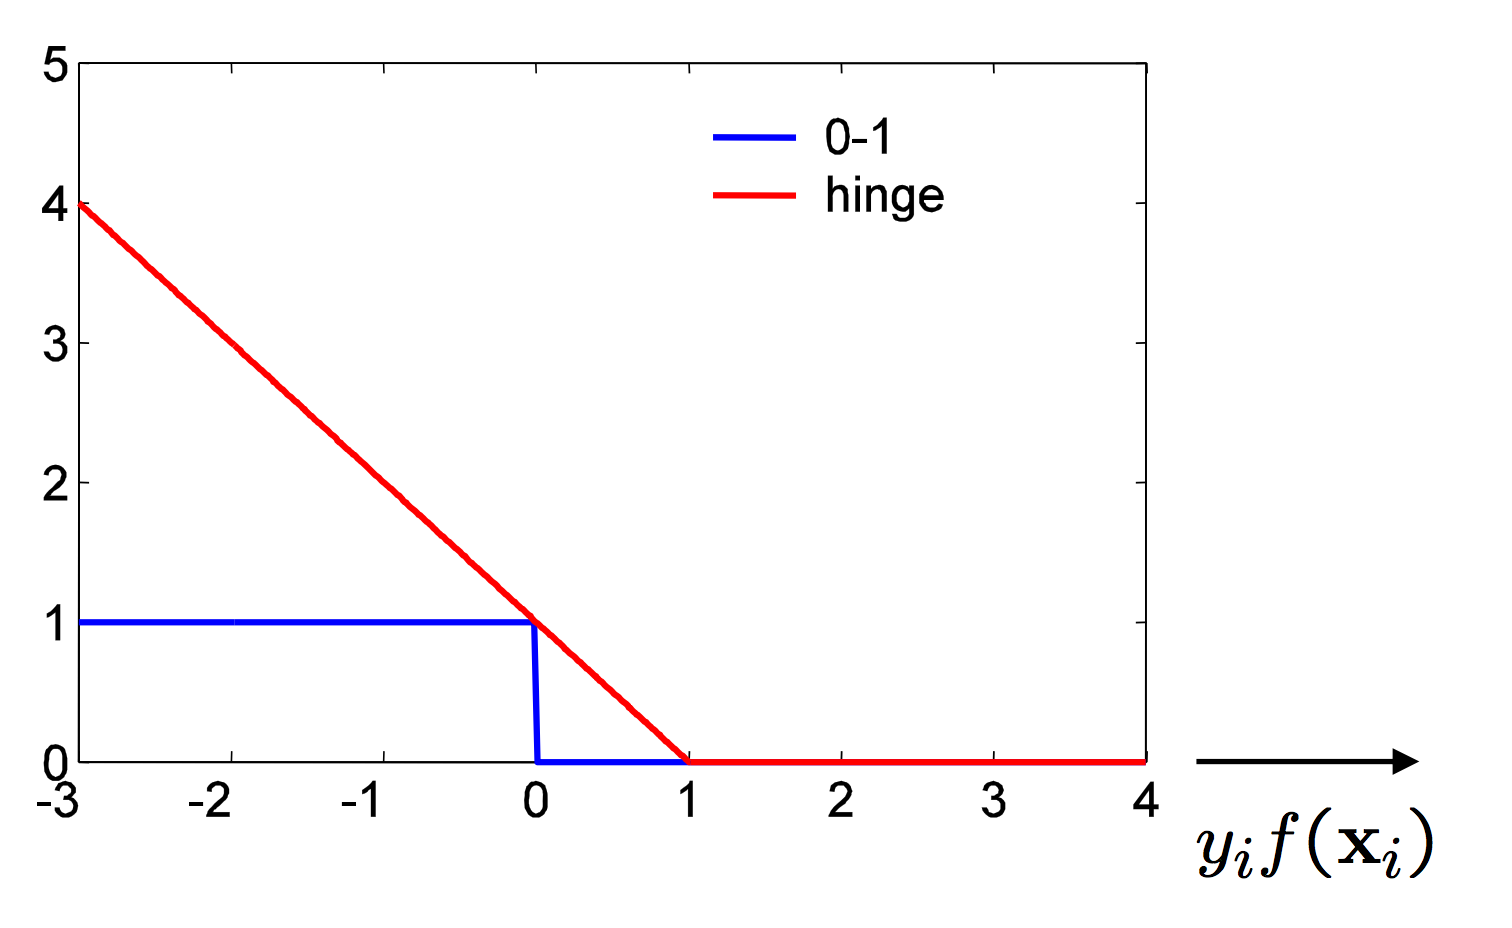
\includegraphics[scale=0.3]{7.png}\\
\textbf{ Figure 2.} Visualization of the hinge loss function 
\end{center}

\subsection{Nonlinear Support Vector Machines with Radial Basis Function Kernel}
\paragraph{}
On the base of linear support vector machine, we now introduce the kernel trick$^{[4]}$ that allows the algorithm to fit the maximum-margin hyperplane in a transformed feature space. Kernels are functions which take low-dimensional input space and transform them into hgher dimensional space i.e. it converts not separable problem to separable problem. There are many different kernel functions developed in the past years. The Radial Basis Function (RBF) kernel is one of the most popular kernels. The RBF kernel on two samples $x$ and $x'$, represented as feature vectors in some input space, is defined as
\[K(x,x') = exp(-\frac{||x-x'||^2}{2\sigma^2}) \]
\paragraph{}
Given the kernel function defined above, we take the Fourier transform of the $K$, and end with a Gaussian Blur function. Therefore, RBF kernel is actually a low-band pass filter, which is a tool to smooth image. It acts as a prior that selects out smooth solutions. Understanding how the kernel does to the data helps us to understand the performance of RBF kernel SVM. 


\section{Experiment}
\paragraph{}
In this section, we demonstrate the implementation of the above algorithms on image classification. Our task in image classification is to predict a category label for a given animal image. Images are 3-dimensional arrays of integers from 0 to 255, of size Width x Height x 3. The 3 represents the three color channels Red, Green, Blue. For the sake of our future implementation, we transferred the RGB into the grayscale image.

\subsection{Data Processing}
\paragraph{}
We used some open-source software libraries to facilitate the implementation, including Scikit-learn (or ‘sklearn’) $^{[6]}$, opencv (Open Source Computer Vision Library)$^{[7]}$, numpy$^{[8]}$,  matplolib, and pickle. Sklearn is a free software machine learning library for the Python. We used the logistic regression, linearSVC, rbf-kernel SVM models in sklearn, and tune the parameters based on our dataset; opencv to read and process the image data; numpy to deal with the image transformed matrix. For performance analysis, matplotlib is useful for data visualization for each model. Pickle plays an important role in saving and loading the trained model for future prediction. With these locally saved model, we created an interactive animal classification that takes in an image use would like to classify as input, the model user would like to use for prediction and returns its predicted category ID.

\subsubsection{Introduction to the COCO dataset}
\paragraph{}
COCO is a popular image recognition, segmentation, and captioning dataset with more than 30,000 images, 2 million instances, and 80 object categories. In this project, we used the 2014 dataset for detection challenge with object instance annotations provided as our primary dataset. For this dataset, there are total 82,782 images of over 90 different categories.
\paragraph{}
The dataset instance annotations are in JSON format, providing comprehensive information. Each annotation instance contains a series of fields, including the category id and segmentation mask of the object, which provides information including the information of the dataset, the category and supercategory of each image belongs to and information about segmentation, etc.
\paragraph{}
In this project, we looked into each annotation instance and created our final dataset using images with supercategory ‘animal.’ For this supercategory in particular, there are ten categories shown as below:
 
\begin{verbatim}
{'id': 16, 'name': 'bird', 'supercategory': 'animal'},
{'id': 17, 'name': 'cat', 'supercategory': 'animal'},
{'id': 18, 'name': 'dog', 'supercategory': 'animal'},
{'id': 19, 'name': 'horse', 'supercategory': 'animal'},
{'id': 20, 'name': 'sheep', 'supercategory': 'animal'},
{'id': 21, 'name': 'cow', 'supercategory': 'animal'},
{'id': 22, 'name': 'elephant', 'supercategory': 'animal'},
{'id': 23, 'name': 'bear', 'supercategory': 'animal'},
{'id': 24, 'name': 'zebra', 'supercategory': 'animal'},
{'id': 25, 'name': 'giraffe', 'supercategory': 'animal'}
\end{verbatim}
 
\subsubsection{Assigning training and testing data sets}
\paragraph{}
Considering the enormous size of the whole dataset, we found it infeasible to train the whole dataset based on the current device we have. Instead, we selected one supercategory 'animal', which contains ten different categories or species shown above. We first extracted all images labeled with $category\_ id$ that belongs to the supercategory 'animals,' which consist of over 19,000 images. After we obtained all animal images, we randomly sample 5,000 images as our final full dimension dataset.
\paragraph{}
We divided the dataset by assigning $3 \slash 4$ of the data, 3750 images, to our training set and the rest of $1\slash 4$, 1250 images, to the testing set. When we sampled the dataset, we shuffled the dataset so that images of most categories under this supercategory are included in the dataset.
 
\subsubsection{Data Feature and Dimension analysis}
\paragraph{}
To process the image and extract the features, we resized all images to size 256 $\times$ 256 so all entries of $X$ have the identical number of pixels. In this case, each image contains 256 $\times$ 256 features. As we discussed above that we split data in the ratio $3:1$, the dimension of training and testing set of $X$ is (3750, 256 $\times$ 256) and (1250, 256 $\times$ 256). The matrix of $X{train}$  would be in the form :
\begin{center}
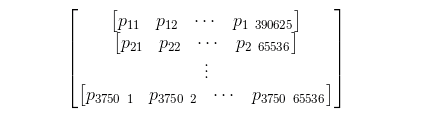
\includegraphics[scale=0.57]{6}
\end{center}
which is a column vector consists of 3,750 row vectors  where $p_{ij}$ is the $j^{th}$ pixel of the $i^{th}$ image in the dataset.
\paragraph{}
Since $Y$ for each $X$ represents the category ID, which is an integer in between 16 and 25, the dimension of training and testing set of $Y$ is (3750, 1) and  (1250, 1) respectively.
 

\subsection{Actual Implementation of Algorithms}
\paragraph{}
In terms of actual implementation, we need to tune the parameters. For multinomial logistic regression, we added an L2 regularization parameter $ \ reg=10\ $ to prevent the case of overfitting. In order to minimize the cost function, we also need to choose the solver to solve this optimization problem. With such large dataset, we tried both the default solver and the solver 'sag,' which uses a stochastic average gradient descent to compute the extremum and learn a true multinomial model. 
\paragraph{}
 For Multilayer Perceptrons neural network, our implementation used the class MLP Classifier in sklearn library. We set the solver as 'adam,' a stochastic gradient-based optimizer$^{[9]}$. We originally set the hidden layer size as (100,100,100), which means that the training model has three hidden layers, each contains 100 neurons. For regularization term, we also added L2 penalty parameter and set it to 0.01.
\paragraph{}
For linear SVM algorithm, since we have 10 categories to classify, SVM need to compute the optimization $45 \times (9 \times 10 \slash 2)$ iterations. In Python, linear SVM is  available in scikit-learn library. We set the penalty parameter C of the error term as $1\slash reg$ (regularization parameter) where $reg = 0.2$, and the loss function is default hinge loss. We use 5,000 labeled data set to train the linear SVM classifier and we will discuss more detailed performance and result in the next section.
 

\section{Performance and Analysis}
\paragraph{}
To evaluate and compare the performance of each algorithm, we computed the training and testing accuracy of prediction of each algorithm. To compare the performance of each algorithm, we plot the confusion matrix as a tool to visualize the result predicted using each model.
\subsection{Evaluate Performance: Confusion Matrix}
\paragraph{}
The confusion matrix helps to visualize the performance of our classifier. To be specific, our classification system has been trained to distinguish between 6 classes: 'birds', 'cat', 'dog', 'horse', 'sheep', and 'cow.' The confusion matrix will summarize the results of testing the algorithm for further inspection. The total number of sample is the sum of all the numbers in the cells. In this confusion matrix, of all the images that are actually in the 'bird' class, 139 are predicted to be in the 'bird' class, 24 are predicted to be in the 'cat' class, 20 are predicted to be in the 'dog' class, 29 are predicted to be in the 'horse' class, 25 are predicted to be in the 'sheep' class and 13 are predicted to be in the 'cow' class. We can see from the matrix that the system has trouble predicting images from class 'cat' and 'dog', but it can  make a pretty good prediction on images from class 'bird', 'sheep' and 'cow'. All correct guesses are located in the diagonal of the matrix, so it's easy to visually inspect the errors from the table as they are represented by values outside the diagonal. The degree of intensity of the color represents the number in each cell. As we can see, a confusion matrix is a straightforward method to visualize the performance of an algorithm.

\subsection{Result and Algorithm Performance} 
\paragraph{}
We reported out the accuracy by training predictors with different models. We trained total six predictors , five of them were trained using 5,000 images with 265 $\times$ 265 pixels and one of them were trained using 1,0000 images downsized to 50 $\times$ 50 features. We wanted to train more predictors using different numbers of neurons per layer with MLP model and over 19,000 images in this dataset. Given the time frame we have for this project, we decided not to do it.

\paragraph{}
The accuracy here is defined as the percentage of the correct category predictions compared to the originally labeled category. Hence, we want the testing accuracy to be closer to the training accuracy. The time elapsed keeps track of the time it took to train each model, which does not include the time used for loading images, testing and saving each model. The accuracy and time elapsed for each algorithm is listed below in Table 1.
\begin{table}[t]
\centering
\caption{Accuracy of Predictor Using Different Algorithm}
\label{my-label}
\begin{tabular}{llll}
\toprule
Algorithm Model & Training Accuracy & Testing Accuracy  &  Time (s) \\
Logistic Regression 1 & 0.9880 & 0.4360 &  1815.84  \\
Logistic Regression 2 & 0.9899 &  0.4200 & 2172.96  \\
MLP 1 & 0.1971 & 0.1952 & 121.34  \\ 
MLP 2 &  0.9669 & 0.4488 & 55.79  \\
Linear SVM & 0.9896 & 0.4240 & 3691.6 \\
Kernel SVM & 0.9909 & 0.4704 &  1522.64 \\
\bottomrule
\end{tabular}
\end{table}
\subsection{Confusion Matrix Analysis}  

\subsubsection{Logistic Regression}

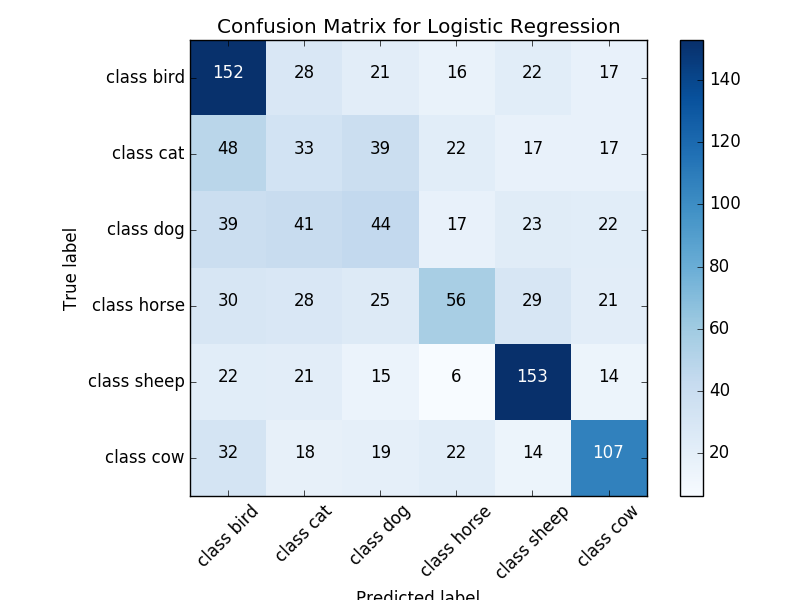
\includegraphics[scale=0.38]{logreg_cm_new.png}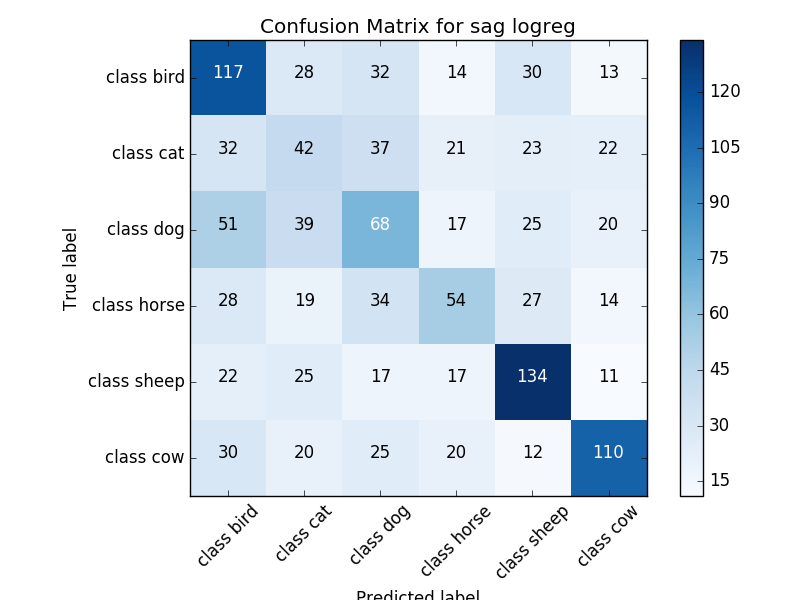
\includegraphics[scale=0.38]{sag_cm_new.png}
\begin{center}
\textbf{Figure 3.a \ Figure 3.b}. Confusion matrices for different solvers of logistic regression.
\end{center}


\paragraph{}
As shown in Figure 3.a, the classifier trained with default solver logistic regression provides a good prediction on bird, cow and sheep category, but cannot distinguish very well between cat, dog and horse. As shown in Figure 3.b, the classifier trained with sag solver logistic regression provides a good prediction on bird, sheep, and cow category. From the graph, we can see that compared with default solver, sag solver provides an averagely better prediction on every class.
 
\subsubsection{Performance of Multilayer Perceptrons}
\paragraph{}
As we discussed above in actual implementation, we set the hidden layer size as (100,100,100), which means we are using 100 neurons per layer to train 256 $\times$ 256 features for each  $X_i$. However, we could see from Table 1 that both training and testing accuracy was not satisfying. The rules-of-thumb of the optimal size of the hidden layer is usually between the size of the input and size of the output layers. We, therefore, increased the layer size and ran another experiment. Due to the the machine's capability, we downsized all images to 25$ \times $ 25 and used a new hidden layer with size (500,500,500).\\\\
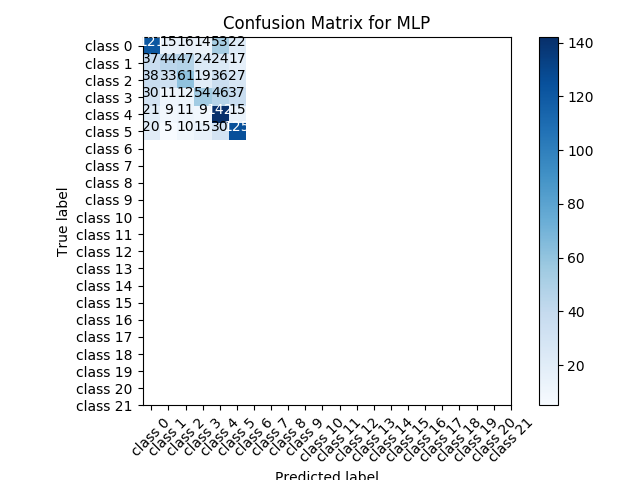
\includegraphics[scale=0.38]{MLP_cm.png}
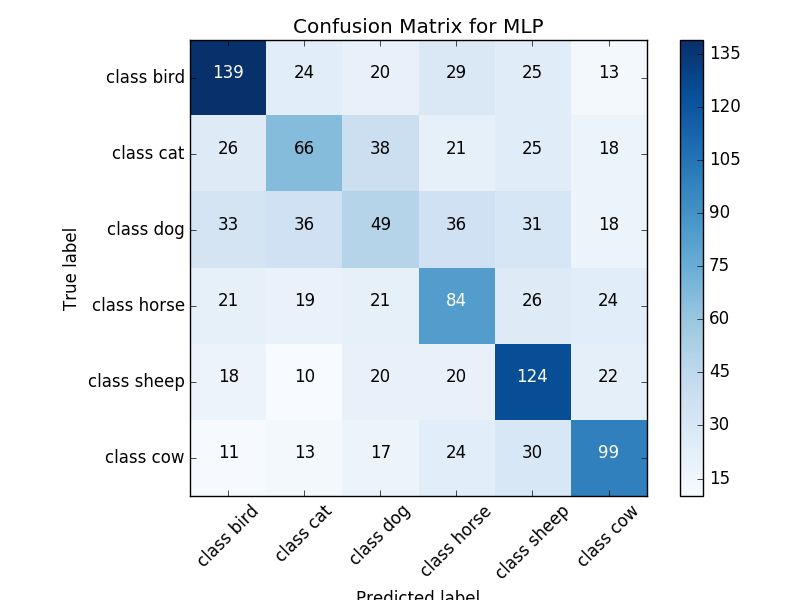
\includegraphics[scale=0.38]{MLP_cm_new1.png}
\begin{center}

\textbf{ Figure 4.a \ Figure 4.b.} Confusion matrices for different parameters of MLP. 
\end{center}
\paragraph{}
From Figure 4.a to Figure 4.b, we can see the effect of tuning parameter correctly. The number of hidden layers and neurons can greatly influence the trained classifier. As shown in Figure 4.a, all true labels are predicted as either dog or horse. We then downsized the image input and increased the number of neurons in each layer, and got a better result as shown in Figure 4.b.
 

\subsubsection{Performance of Linear and Kernel SVM}
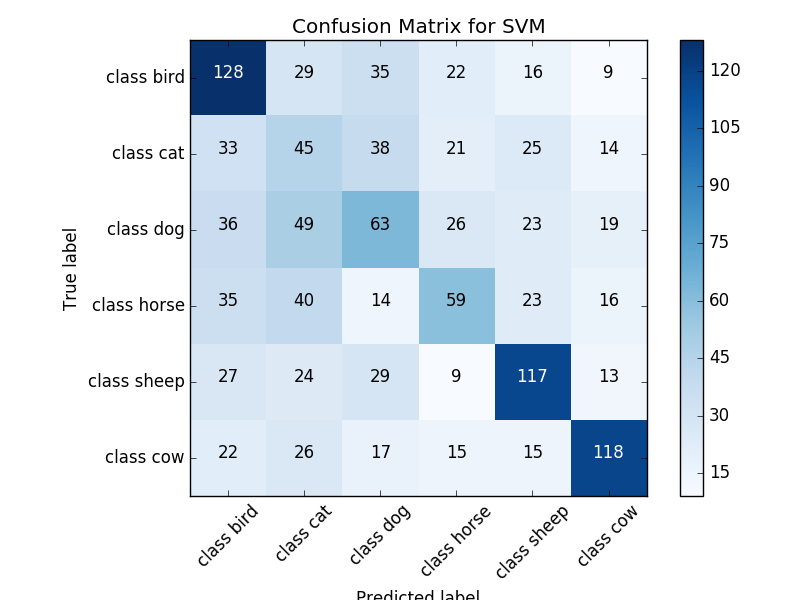
\includegraphics[scale=0.38]{svm_cm_new.png}
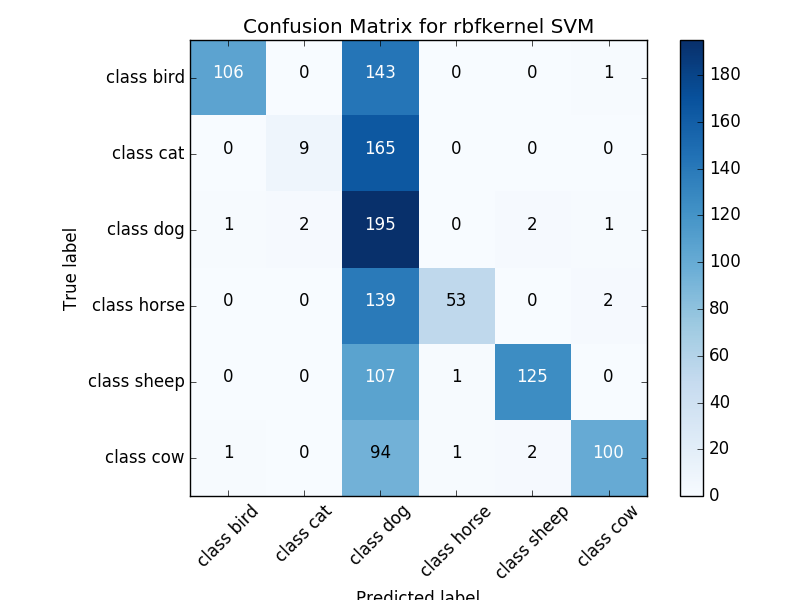
\includegraphics[scale=0.38]{kernelSVM_cm_new.png}
\begin{center}
\textbf{ Figure 5.a \ Figure 5.b.} Confusion matrices for SVM with different kernels.

\end{center}
\paragraph{}
As shown in Figure 5.a, the classifier trained with linear SVM provides a good prediction on bird, sheep and cow category. Due to the larger number of images labeled with 'cat', 'dog' and 'horse', and the presence of people in those images, it is difficult for linear SVM to predict images from class 'dog', 'cat' and 'horse' correctly. On the other hand, the classifier trained with RBF-kernel SVM as shown in Figure 5.b, predicts most of the images to be either in the class 'dog', or their true labels. For instance, for images labeled with 'bird', it can be either predicted as 'dog' or 'bird.' We consider this result interesting and worth to do future research on.

 

\section{Conclusion}
\paragraph{}
To summarize, we proposed multiple methods for object classification and evaluated and compared the performance of each method through different experiments on species categories on animal image data. We train an animal category predictor using logistic regression model, multilayer perceptrons neural network, support vector machines (SVM) with linear kernel and radial basis function kernel, which could be output and saved on disk. In terms of runtime, the multilayer perceptrons algorithm has a significant advantage. In terms of accuracy, kernel SVM reaches 47$\%$ and MLP reaches 45$\%$ of accuracy. Overall, multilayer perceptron neural network stands out and has great potential in the future.
 

\section{Future Work}
\paragraph{} 
Due to the limitation of our laptop memory, we cannot use a more complicated neural network to train our data. Based on the result of our current model, it is promising to have better accuracy if we improve the number of neurons and train larger dataset, which will require running the code on GPU. Moreover, we need to tune the parameters. For instance, the regularization parameter, the number of layers and neurons, and different random weight initializations for a better result. 

\section*{Acknowledgement}
We would like to thank Prof.Gu and our grutors Maggie and Zhepei for their help throughout this course.

\section*{References}
\small
[1] COCO, Common Objects in Context, \url{http://mscoco.org/dataset}

[2] Vapnik,\ V., Golowich,\ S.\ E., \& Smola,\ A.\ J. (1997). Support vector method for function approximation, regression estimation and signal processing. In Advances in neural information processing systems (pp. 281-287). 

[3] Chang, Y.\ W., Hsieh, C.\ J., Chang, K.\ W., Ringgaard, M., \& Lin, C.\ J. (2010). Training and testing low-degree polynomial data mappings via linear SVM. Journal of Machine Learning Research, 11(Apr), 1471-1490. 

[4]   Aizerman, Mark A.; Braverman, Emmanuel M.\ \& Rozonoer, Lev I.\ (1964). "Theoretical foundations of the potential function method in pattern recognition learning". Automation and Remote Control. 25: 821-837.

[5] Haykin,\  S., \ \& Network, N. (2004). A comprehensive foundation. Neural Networks, 2(2004), 41.

[6] Van der Walt, S., Schönberger, J. L., Nunez-Iglesias, J., Boulogne, F., Warner, J. D., Yager, N., ... \& Yu, T. (2014). scikit-image: image processing in Python. PeerJ, 2, e453.

[7] Bradski, G., $\&$ Kaehler, A. (2008). Learning OpenCV: Computer vision with the OpenCV library. " O'Reilly Media, Inc.".

[8] Walt, S. V. D., Colbert, S. C., $\&$ Varoquaux, G. (2011). The NumPy array: a structure for efficient numerical computation. Computing in Science $\&$ Engineering, 13(2), 22-30.

[9] Kingma, D., $\&$ Ba, J. (2014). Adam: A method for stochastic optimization. arXiv preprint arXiv:1412.6980.


\end{document}